\documentclass[journal]{IEEEtran}
\usepackage[utf8]{inputenc}
\usepackage[official]{eurosym}
\usepackage{csquotes}
\usepackage{graphicx}

\usepackage{tikz}
\usetikzlibrary{automata,backgrounds,shapes,matrix,arrows,decorations.pathmorphing}

\usepackage{amsmath,amsfonts,amssymb}
\usepackage{bm}
\usepackage{mathtools}


\usepackage{algorithm}
\usepackage{algpseudocode}
\algblock{Input}{EndInput}
\algnotext{EndInput}
\algblock{Output}{EndOutput}
\algnotext{EndOutput}
\makeatletter
\newenvironment{pseudocode}[1][htb]{%
    \renewcommand{\ALG@name}{Pseudocode}% Update algorithm name
   \begin{algorithm}[#1]%
  }{\end{algorithm}}
\makeatother

% % \usepackage[dvipsnames]{xcolor}
% \definecolor{CrispBlue}{HTML}{0176AE}
% \usepackage{tcolorbox}
% \usepackage{etoolbox}
% \BeforeBeginEnvironment{verbatim*}{\begin{tcolorbox}[colback=CrispBlue!5!white,colframe=CrispBlue!75!black]}%
% \AfterEndEnvironment{verbatim*}{\end{tcolorbox}}%

\usepackage{lipsum}
% \usepackage[caption=false, font=footnotesize]{subfig}
\graphicspath{ {./graphics/} }
\hyphenation{op-tical net-works semi-conduc-tor}

\begin{document}
\title{Gaussian Process Networks for Machine Learning}% <-this % stops a space

\author{David~Kirby,~\IEEEmembership{Student Member,~IEEE}%
\thanks{The author is with the Department of Electrical and Computer Engineering, University of New Mexico, Albuquerque, NM 87131 USA (e-mail: davidkirby@unm.edu).}%
}

\maketitle
\begin{abstract}
    This paper describes the basic nomenclature and ideas behind Gaussian process networks as they apply to machine learning, including a summary of linear Gaussian processes, Gaussian processes in Reproducing (Recursive) Kernel Hilbert Spaces, and inference over hyperparameters. It then goes into experiments of the linear Gaussian process as well as the nonlinear Gaussian process. It briefly introduces the signal model and the optimization criterion used in Gaussian Processes for the case of linear processes. Provides the RKHS model for a Gaussian process. Fully develops the dual expression for the posterior and the likelihood models of the Gaussian process. Proves that the kernel matrix is actually a covariance matrix.
\end{abstract}
\begin{IEEEkeywords}
    Gaussian Process, Statistical Learning Theory, Machine Learning, Linear Gaussian, Nonlinear Gaussian.
\end{IEEEkeywords}

% ************************************************************************************
\section{Introduction}

\IEEEPARstart{T}{he} difference between the Gaussian process networks and other methods that we have used this semester is the criterion that we are going to use to optimize our estimators; ones based on Bayes' Rule. To understand Bayes' Rule in full, we need to first look at what is a conditional probability distribution; let us do it with a classic diagram. We have a space that is often called the universe of probability or sample space (\(\Omega\)) and it represents in its coordinates all possible outcomes of an observation. Let us say for example we have three coins and we toss them, with some heads and some tails, this would give us \(2^3=8\) possible events. Let's define a given event, say a combination of tails, we will call it event \(A\), and another event \(B\). If we examine these two events, they can overlap. There are situations at which both events happen at the same time, and times when when do not. If, for example, we know the probability of \(A\) (i.e., we know the physics of the phenomenon, three coins that are perfectly symmetrical, then the probability of heads or tails is \(\frac{1}{2}\)), then we can calculate all the possible events and their probabilities before we do the experiment. This is called \textit{a priori}, a Latin phrase meaning `from the earlier'.

\begin{figure}[ht]
    \centering
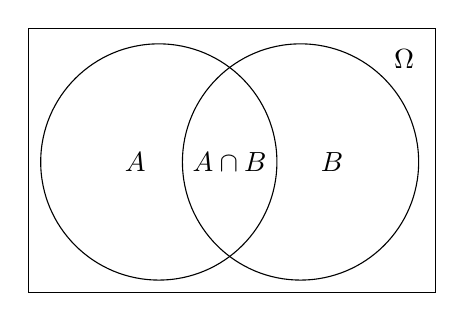
\begin{tikzpicture}
    [show background rectangle]
    % Set A
    \node [draw,
        circle,
        minimum size =3cm]
        (A) at (0,0){};
     
    % Set B
    \node [draw,
        circle,
        minimum size =3cm,
        label={45:$\Omega$}] (B) at (1.8,0){};
     
    % Set intersection label
    \node at (0.9,0) {$A\cap B$};
    \node at (-0.3,0) {$A$};
    \node at (2.2,0) {$B$};
\end{tikzpicture}
\caption{Universe of probability with two events.}
\label{fig:Bayes}
\end{figure}

Bayes' Rule or Bayes' Theorem, takes these probabilities even further. What if, for example, we are given information on one of the events? If we have knowledge about one of the events, the probability will change (and actually increase because the universe of probabilities \(\Omega\) has been reduced). If event B happens, the universe of probabilities collapses to the area defined by \(B\). Then, given that \(A\) is a prior, \(B\) is an observation (knowledge), and we know the probability of \(B\), we can determine the probability of \(A\) given \(B\).
\begin{align}
    P&(A\big|B) = \frac{P(A\cap B)}{P(B)},\\
    \notag&\text{where }P(A\cap B) \text{ is a joint probability.}
\end{align}

Since \(A\) is not observable, this is useful as the probability of \(A\) given \(B\) is a posterior (i.e., a probability after the observation). \(P(B)\) then is our marginal likelihood and \(P(B|A)\) is our likelihood. In summary, posterior is proportional to the likelihood times the prior. Maximizing this is called \textit{maximum a posteriori} and if we maximize this likelihood \(P(B|A)\) with respect to \(A\), and then choose the corresponding value of \(A\), we can find the maximum likelihood. Using both of these criterion: maximization of a posterior and maximization of our likelihood, we will have everything we need in order to start to construct the Gaussian processes.


% ************************************************************************************
\section{Theory}

\subsection{Linear Gaussian Processes}

Gaussian processes (GPs) need a probabilistic model for the latent variable for what we want to infer. This Bayesian inference is a change from our previous lectures since we no longer need to cross-validate any parameters because all of the parameters will be optimized by maximum posteriori and maximum likelihood. Cross-validating models can be fickle, but the catch is that we need a model for the data, which was not true for support vector machines. The question then is how do we translate the Bayesian inference to machine learning? We have some observation \(\mathbf{x}\) and with this observation we want to infer the value of the label \(y\) or the order of the regressor and we do this using the Bayesian perspective, a probabilistic framework.

We have a random variable \(\mathbf{w}\) which is our set of parameters of the model and we have \(y=\mathbf{w}^\top \mathbf{x}\). \(\mathbf{w}\) is the latent variable that we can neither observe nor adjust as before; however, we can do inference on it. During a training, we have a set of observations \(\mathbf{x}\) and \(y\), but during a test, \(y\) is not observable. We have \(y\) and \(\mathbf{x}\) as knowledge and what we want to do is to compute the probability of \(\mathbf{w}\) given the knowledge of \(y\) and \(\mathbf{x}\); this is a posterior probability. By applying Bayes' Rule, we can say the probability of \(\mathbf{w}\) given \(\mathbf{x}\) and \(y\) is equal to the probability of \(\mathbf{x}\) and \(y\) given \(\mathbf{w}\).
\begin{equation}
    P(\mathbf{w}\big|y,\mathbf{x}) = \frac{P(\mathbf{w}\cap y,\mathbf{x})}{P(y,\mathbf{x})}
\end{equation}

An important thing to note is that conditional probability is still probability; therefore, it must have the same properties of non-conditional probability. With this in mind, and using our statement earlier that the posterior is proportional to the likelihood times the prior, we can say that the probability of \(\mathbf{w}\) given \(\mathbf{x}\) and \(y\) is proportional to the probability of \(y\) given \(\mathbf{x}\) and \(\mathbf{w}\) times the probability of \(\mathbf{w}\).
\begin{equation}
    P(\mathbf{w}\big|y,\mathbf{x}) \propto P(y\big|\mathbf{x},\mathbf{w})P(\mathbf{w})
\end{equation}

Analyzing our estimation model, we take \(\mathbf{x}\) and input it into a machine that has a set of parameters \(\mathbf{w}\) and obtain an estimation \(y\). It turns out that \(y\) will change depending on different values of \(\mathbf{w}\). These different values are the error and our goal is to minimize this error. The output will depend on \(\mathbf{w}\), but the input \(\mathbf{x}\) does not depend on \(\mathbf{w}\) because \(\mathbf{x}\) is given and does not change. One of the properties of this independence is that the probability of \(\mathbf{x}\) and \(\mathbf{w}\) is equal to the product of their individual probabilities.

Ultimately, we want to compute the probability of \(y\) given something that we already know \(\mathbf{x}\) and something that we do not know \(\mathbf{w}\). We want to maximize this probability given an observation. To do this, we need to modify \(\mathbf{w}\) in order to maximize the posterior probability. The point of GPs is that we do not use the maximum a posteriori of \(\mathbf{w}\), but use the posterior, the whole probability distribution, and we use this probability distribution to compute the posterior probability of a regressor during the test. Once we have this posterior we use it maximize the posterior probability given an observation during a test. More than that, we do not keep the maximum posteriori, we keep the posterior probability of our latent variable \(y\), the estimation given the input data and given the training data. This is important because in our previous models (SVM) we had a function \(y = \mathbf{w}^\top \mathbf{x}\) where we inferred particular values for \(\mathbf{w}\), and we had multiple values for \(y\), which is the estimation. Here, instead of using \(\mathbf{w}\), we use the probability distribution of \(\mathbf{w}\) and we will obtain a probability distribution for our estimation as well. This probability distribution will be Gaussian which means that we can find a mean and a variance. The mean will be our prediction and the variance will be our predictive confidence interval of our prediction. If the confidence interval is small (tight), then our prediction is good; if our confidence interval is high (wide), then our prediction is not possible. This is a better solution because not only do we now have a machine that tells us a prediction, but is also telling us whether or not to trust that prediction. These machines are optimal for models where the data is Gaussian, but worse than other machines for non-Gaussian data.

\subsection{Gaussian Processes in Recursive Kernel Hilbert Spaces}

The Bayesian inference model that we looked at in the previous section gave us a posterior distribution based on given observations. From there we can move into regression models and see that this method can be kernelized. We insert the representative theorem inside and work with the dual expression to get an alternative for GPs that are nonlinear but still keep all of the properties of GPs, in particular we can have a maximum a posteriori for our model, we can have a maximum a posteriori for our prediction, and in this maximal posteriori, if it is Gaussian, then we have a mean and a variance as well.

To develop the dual expression for the posterior and the likelihood models of the GP, we begin with the model of:
\begin{align}
    y_n &= \mathbf{w}^\top \mathbf{x}_n + \epsilon_n
\end{align}
where \(y_n\) is a column vector, \(\mathbf{x}_n\) is a matrix containing all of the input data, \(\mathbf{w}\) contains our bias \(b\), and \(\epsilon_n\) is a random variable which is i.i.d. and Gaussian. This error is drawn from a normal Gauassian with zero mean and a variance \(\sigma_n^2\). Though we do not know \(\sigma_n^2\), we do know that it is the same for all values of \(n\), and given this we know that \(y_n\) is drawn from another normal \(y_n\) given a mean \(\mathbf{w}^\top \mathbf{x}_n\) and variance exactly equal to the variance of \(\epsilon\). This means that we also know that \(y_n\) is conditionally i.i.d. and if we know \(\mathbf{w}\) the values of \(y)n\) become independent.

Since \(y_n\) is conditionally independent, then the distribution of \(y_n\) is equal to the product of the distributions and the product of identical Gaussians will produce another Gaussian, this one multivariate. It is a Gaussian of all the elements of the sequence and its mean then is \(\mathbf{x}_n^\top \mathbf{w}\) and variance \(\sigma_n^2 \mathbf{I}\). Since \(\mathbf{w}\) is a random variable, we can model with a Gaussian with zero mean and a covariance that we will call \(\Sigma_p\). Recall that \(\mathbf{w}\) is our prior) and \(\mathbf{y}\) is now our likelihood, though it is now a vector. With this we can compute the posterior distribution of the model:
\begin{align}
    &\mathbf{w} \big| \mathbf{X}, \mathbf{y} \sim \mathcal{N}(\mathbf{w}\big| \overline{\mathbf{w}}, \mathbf{A}^{-1})\\
    \notag\text{where: }\\
    \mathbf{A} &= \sigma_n^{-2}\mathbf{X}\mathbf{X}^\top + \Sigma_p^{-1}\label{eq6}\\
    \overline{\mathbf{w}} &= \left(\mathbf{X}\mathbf{X}^\top + \sigma_n^{2}\Sigma_p^{-1}\right)^{-1}\mathbf{X}\mathbf{y}\label{eq7}
\end{align}
This is again proportional to the likelihood times the prior. Where \(\mathbf{A}\) is the inverse of the covariance matrix and \(\overline{\mathbf{w}}\) is the mean and is our maximum a posteriori solution for \(\mathbf{w}\). This is similar to the ridge regression we have seen in other models. Finally, we do not want a solution that contains a maximum a posteriori, we want a solution that contains the posterior. We compute:
\begin{align}
    P(f_* \big| \mathbf{x}^*,\mathbf{y},\mathbf{X})
\end{align}
where \(\mathbf{x}^*\) is the test sample and \(f_*\) is what is called a latent function (similar to our latent variable in the previous section). While we do not know \(f_*\), we can find its probability distribution by taking the integral w.r.t. \(\mathbf{w}\). This solution is a Gaussian:
\begin{align}
    \mathcal{N}\left(f_*\big| \overline{\mathbf{w}}^\top \mathbf{x}^*, {\mathbf{x}^*}^\top \mathbf{A}^{-1}\mathbf{x}^*\right)
\end{align}
Now that we have completed this in the primal space, we apply the representer theorem to go to dual space and then Mercer's theroem to obtain a kernel. By expressing \(\mathbf{w}\) as a linear combination of the data (\(\alpha\), and replacing \(\mathbf{X}\) with \(\mathbf{\Phi}\) in equations~(\ref{eq6}) and~(\ref{eq7}), the solution contains only dot products between samples. This finally gives us a pure, nonlinear GP with a mean and a variance for the solution prediction, plus a new interpretation of this covariance. Taking the transformed equations, we use Mercer's Theorem, which states that if \(k (\mathbf{x}_n, \mathbf{x}_m)\) exists, gives a real number, and is positive-definite, then it is a dot product in the Hilbert space and we can say:
\begin{equation}
    k (\mathbf{x}_i, \mathbf{x}_j) = <\phi^\top(\mathbf{x}_i) \Sigma_p \phi (\mathbf{x}_j)>
\end{equation}

This dot product in the Hilbert space can be expressed as a function of the vectors in the input space, no longer dependent on \(\Phi\). In support vector machines, we needed to go to dual, then once we were there, we needed to apply quadratic programming; however, here we just need to invert the matrix. In ridge regression we needed to sweep \(\sigma\) in order to find \(\gamma\); in GPs, we do not need to do any cross-validation. This saves an incredible amount of computational time, but there is no free lunch and this solution is not unique and we need a Gaussian model.

\subsection{Inference Over the Hyperparameters}
Hyperparameters can constructively or adversly affect the regression model and should be chosen accordingly to optimize performance. The following pseudocode, taken from Rasmussen~\cite{Rasmussen} shows the optimization of the hyperparameters of a GP using exact inference.

\begin{pseudocode}
    \caption{Optimization of the hyperparameters of a GP}
    \begin{algorithmic}[1]
    \Input{ : }{ \(X\) (inputs)}{ \(\mathbf{y}\) (\(\pm1\) targets) }{\(\bm{\theta}\) (hyperparameters)}
    \State compute \(K\) 
    
    \quad(compute covariance matrix from \(X\) \& \(\bm{\theta}\))
    \State (\(\bm{\tilde{\nu}}, \bm{\tilde{\tau}}, \log{Z_{\text{EP}}}\)) := EP (\(K, \mathbf{y}\))

    \quad(run the EP Algorithm)
    \State \(L :=\) cholesky (\(I + \tilde{S}^{\frac{1}{2}}K\tilde{S}^{\frac{1}{2}}\))

    \quad(solve \(LL^\top = B = I + \tilde{S}^{\frac{1}{2}}K\tilde{S}^{\frac{1}{2}}\))
    \State \(\mathbf{b}:= \bm{\tilde{\nu}} - \tilde{S}^{\frac{1}{2}} L \backslash (L^\top \backslash \tilde{S}^{\frac{1}{2}} K \bm{\tilde{\nu}})\)

    \quad(\(\mathbf{b}\) from under eq. (5.27))
    \State \(R := \mathbf{bb}^\top - \tilde{S}^{\frac{1}{2}} L^\top \backslash (L \backslash \tilde{S}^{\frac{1}{2}} )\)

    \quad (\(R = \mathbf{bb}^\top - \tilde{S}^{\frac{1}{2}} B^{-1} \tilde{S}^{\frac{1}{2}} \))
    \For {\(j := 1 \dots \dim{(\bm{\theta})} \)}
    
        \(C := \partial{K} / \partial{\theta_j} \)

        \quad (compute derivative matrix from \(X\) \& \(\bm{\theta}\))

        \( \nabla_j \log{Z_\text{EP}} := \frac{1}{2}\ tr(RC) \)

        \quad (eq. (5.27))
    \EndFor
    \EndInput
    \Return{: }{\(\log{Z_\text{EP}}\)}, (log marginal likelihood), \( \nabla \log{Z_\text{EP}}\) (partial derivatives)
    \end{algorithmic}
\end{pseudocode}

% ************************************************************************************
\section{Experiments}

\subsection{Linear Gaussian Process}
\subsubsection{Experimental Setup}
\paragraph{\normalfont{Generate an ARMA process with}}
\begin{align*}
    &\text{moving average (MA) coefficients}\\
    \mathbf{b} &= \{0.0048, 0.0193, 0.0289, 0.0193, 0.0048\}^ \top\\
    &\text{and auto-regressive coefficients}\\
    \mathbf{a} &= \{1, -2.3695, 2.3140, -1.0547, 0.1874\}^ \top
\end{align*}
\paragraph{\normalfont{Generate a process input \(x[n]\) consisting of 100 samples \( (1 \le n \le 100) \) of Gaussian noise with unit variance and zero mean. Choose a uniformly distributed random subset of 20 samples of the process output \(f[n]\) as training set}}

\begin{figure}[ht!]
    \centering
    \includegraphics[width=\linewidth]{figure02.png}
    \caption{Linear Gaussian Process for Prediction Using ARMA Process with given parameters.}
    \label{fig:fig02}
\end{figure}

\subsubsection{Linear Gaussian Process for Prediction}
\paragraph{\normalfont{Using MATLAB, we constructed a linear Gaussian process for which the input is defined as \( x[n] = n\), and the output is \(f[n]\). Using a dual (a.k.a. feature space) formulation in the code. Representing the predicted values for \( (1 \le n \le 100) \), together with its variance, we then compared the result with the real values of the ARMA model obtained in the experimental setup}}

\subsubsection{Linear ARMA with AR(1) process noise}
\paragraph{\normalfont{Constructed an ARMA process equal to the previous one, and added an AR(1) noise of parameter \(a_n = 0.2\) process to the output \(f[n]\), this is, to construct the output}}

\begin{align*}
    y[n] &= f[n] + g[n]\\
    \text{where } g[n] &= w_g[n] + 0.2g[n-1]\\
    \text{and } w_g[n] &\text{ is white noise of variance 0.1}
\end{align*}

\begin{figure}[ht!]
    \centering
    \includegraphics[width=\linewidth]{figure03.png}
    \caption{Linear Gaussian Process With High Dimension.}
    \label{fig:fig03}
\end{figure}

\paragraph{\normalfont{Constructed a model that exactly matches the process \(f[n]\), this is}}

\begin{align*}
    f[n] &= \mathbf{a}^\top \mathbf{f}[n-1] + \mathbf{b}^\top \bm{\omega}[n-1] = \mathbf{w}^\top \mathbf{x}[n]
\end{align*}

\noindent where \(\mathbf{f}[n-1]\) and \(\bm{\omega}[n-1]\) are vectors constructed with the \({n-1}^{th}\) to \({n-5}^{th}\) samples of the input and output processes.

\begin{figure}[ht!]
    \centering
    \includegraphics[width=\linewidth]{figure05.png}
    \caption{Linear Gaussian Process That Exactly Matches the Process \(f[n]\).}
    \label{fig:fig05}
\end{figure}

\begin{figure}[ht!]
    \centering
    \includegraphics[width=\linewidth]{figure04.png}
    \caption{Nonlinear Gaussian Process with White Noise.}
    \label{fig:fig04}
\end{figure}

\paragraph{\normalfont{Computed the theoretical value of the output covariance matrix, using it to construct a Gaussian process to optimize parameter \(\mathbf{w}\) using 100 samples of the data and compared the results with the actual parameters}}

\paragraph{\normalfont{Tested the model with another 100 samples of the data, representing the predictive mean and the predictive mean with \(\pm 2\) standard deviations}}

\subsection{Nonlinear Gaussian Process}
If the ARMA model is approximated using a small FIR filter of the output, the expected performance will be poor. As an example, we reproduced the previous experiment, but modifying the input so it only contains the last five values of \(x[n]\) (i.e., removing \(\mathbf{f}[n]\) from the model). Using a nonlinear model will improve the performance.

\paragraph{\normalfont{Using the GPN software included in our textbook, we constructed a predictor of \(y[n]\) that uses only the input values \(\mathbf{x}[n]\) and a covariance matrix consisting of the sum of a square exponential plus a noise matrix. Let the software figure out the hyperparameters using the exact inference methods for two cases}}

\begin{itemize}
    \item With an output \(f[n]\) corrupted by the white plus AR(1) noise of the section above.
    \item With only white noise.
\end{itemize}



% \begin{figure}[ht]
%     \centering
%     \includegraphics[width=\linewidth]{figure05.png}
%     \caption{Fifty datapoints with \( \sigma = 0.2\).}
%     \label{fig:data1}
% \end{figure}

\section{Discussion}

This paper was designed to describe the basic nomenclature and ideas behind Gaussian process networks as they apply to machine learning, including a summary of linear Gaussian processes, Gaussian processes in Reproducing Kernel Hilbert Spaces, and inference over hyperparameters. It explored  experiments of the linear Gaussian process as well as the nonlinear Gaussian process. It briefly introduced the signal model and the optimization criterion used in Gaussian Processes for the case of linear processes. Provided the RKHS model for a Gaussian process. Fully developed the dual expression for the posterior and the likelihood models of the Gaussian process and proved that the kernel matrix is actually a covariance matrix.

\section*{Acknowledgment}
The author would like to thank the University of New Mexico for the generous access to research material, as well as Dr. Manel Martínez-Ramòn for the opportunity to explore Machine Learning and Gaussian Processes.

\begin{thebibliography}{6}
\bibstyle{IEEEtran}

\bibitem{Rasmussen}
C.~E.~Rasmussen and C.~Williams, \textit{\enquote{Gaussian Processes for Machine Learning}}, MIT Press, 2006.

\bibitem{Stat}
T.~Hastie, R.~Tibshirani and J.~Friedman, \textit{\enquote{The Elements of Statistical Learning: Data Mining, Inference, and Prediction,}} 2nd ed., Springer, 1998.

\end{thebibliography}

\end{document}
